\documentclass[11pt]{article}
\usepackage[letterpaper,margin=0.9in]{geometry}
\usepackage[hidelinks]{hyperref}
\usepackage{enumitem}
\usepackage{titlesec}
\usepackage{tabularx}
\usepackage{graphicx}

\setlist[itemize]{leftmargin=1.2em,itemsep=3pt,topsep=3pt}
\titleformat{\section}{\large\bfseries}{}{0em}{}[\titlerule]

\newcommand{\entry}[4]{
  \noindent\begin{tabularx}{\textwidth}{@{}Xr@{}}
    \textbf{#1} & #2 \\
    \textit{#3} & \textit{#4}
  \end{tabularx}\vspace{2pt}
}

\begin{document}

\noindent\begin{minipage}[t]{0.76\textwidth}
\vspace{0pt}
{\LARGE \textbf{Piter Z. Garcia Bautista}}\\[4pt]
Rochester, NY \textbar\ +1 (646) 288-3300 \textbar\ \href{mailto:pzg8794@rit.edu}{pzg8794@rit.edu}\\
\href{https://linkedin.com/in/garciapiterz}{linkedin.com/in/garciapiterz} \textbar\
\href{https://github.com/pzg8794}{github.com/pzg8794} \textbar\
\href{https://garciapiterz.com}{garciapiterz.com}
\end{minipage}%
\hfill\begin{minipage}[t]{0.20\textwidth}
\vspace{0pt}
\raggedleft
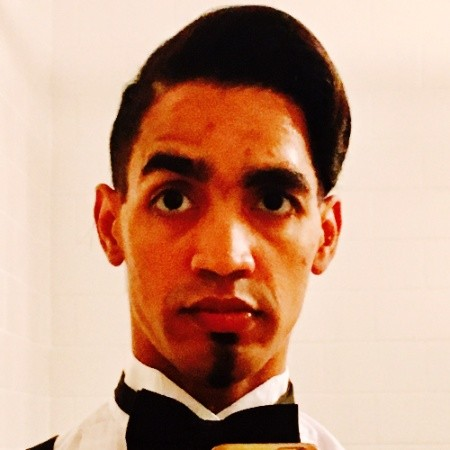
\includegraphics[width=\linewidth]{profile_pic}
\end{minipage}
\vspace{6pt}

\section{Research Profile}
Graduate researcher focused on machine learning under uncertainty, noisy observations, and limited-signal environments. Background spans reproducible ML evaluation pipelines, bandit and reinforcement-learning-based decision-making systems, quantum computing research, and fault-tolerant algorithm design. Current Graduate Assistant work (Quantum and AI Research, RIT) emphasizes reliability-first evaluation methodology, structured experimental design, and principled approaches to settings where standard supervised assumptions break down. Particularly interested in how statistical learning can be made robust and trustworthy in noisy physical and computational systems, including quantum circuits.

\section{Research Interests}
Reliable machine learning under noise and uncertainty; fault-tolerant algorithm evaluation; quantum computing and quantum-classical hybrid methods; bandit learning and sequential decision-making; reproducible benchmarking and structured experimental design.

\section{Education}

\entry{Rochester Institute of Technology}{Expected Aug 2026}{Master of Science, Data Science --- GPA 3.9}{Rochester, NY}
\begin{itemize}
  \item Concentration: Bioinformatics \& Artificial Intelligence.
  \item Relevant coursework: Data-Driven Knowledge Discovery, Neural Networks \& Deep Learning, Applied Data Science, Bioinformatics Algorithms, Software Engineering for Data Science.
\end{itemize}

\entry{University of Rochester, Warner School of Education}{In progress}{Graduate study, Teaching Computer Science K--12 (M.S. track) --- GPA 4.0}{Rochester, NY}
\begin{itemize}
  \item NSF Robert Noyce Scholar (\$30,000 full funding); Advanced Certificate in Leadership in Disability and Inclusive Practices.
\end{itemize}

\entry{Rochester Institute of Technology}{2015}{Master of Science, Computer Science --- GPA 3.2}{Rochester, NY}
\begin{itemize}
  \item Concentrations: Artificial Intelligence, Big Data Analytics, Computer Graphics.
  \item MS Thesis: ASL Recognition Application --- image processing and pattern recognition under partial-observation constraints.
\end{itemize}

\entry{Farmingdale State College}{2012}{Bachelor of Science, Computer Engineering --- GPA 3.3}{Farmingdale, NY}
\begin{itemize}
  \item Dual degree: Electrical Engineering \& Computer Engineering Technology.
  \item Honors: CSTEP Award \& Merit; Dual BS Scholarship.
\end{itemize}

\section{Research and Professional Experience}

\entry{Rochester Institute of Technology, Software Engineering Department}{Fall 2025 -- Present}{Graduate Assistant, Quantum and AI Research}{Rochester, NY}
\begin{itemize}
  \item Build reproducible ML evaluation pipelines across local, Colab, and GCP environments for quantum-adjacent algorithmic experiments, with structured logging and failure-mode tracking.
  \item Apply bandit-style exploration and sequential decision-making to quantum circuit routing under hardware noise, developing adaptive resource allocation strategies for NISQ-era reliability constraints.
  \item Co-author manuscript-level technical analyses on quantum path optimization and fault-tolerant routing under noise constraints; currently under submission.
  \item Design evaluation frameworks that isolate algorithmic reliability from environmental noise, enabling clean comparison between quantum-classical hybrid approaches.
\end{itemize}

\entry{University of Rochester, Warner School of Education}{Sep 2024 -- Present}{CS Teacher Candidate \& Education Research (NSF Noyce Scholar)}{Rochester, NY}
\begin{itemize}
  \item Deliver K--12 computer science instruction in active public school placement as part of the NSF Robert Noyce Scholar program, including computational thinking, inclusive pedagogy, and NYS learning standards.
  \item Conduct applied education research on AI-informed and data-driven approaches to improve learning outcomes for neurodivergent students, applying Universal Design for Learning (UDL) and evidence-based adaptive strategies.
  \item Produce lesson artifacts and instructional analyses documenting the intersection of AI, inclusive education, and evidence-based CS pedagogy.
\end{itemize}

\entry{Rochester Institute of Technology}{2024 -- 2025}{Equitable Bioinformatics Research --- ISTE-780}{Rochester, NY}
\begin{itemize}
  \item Pioneered fairness assessment applied to RNA secondary structure prediction algorithms, implementing bias-detection frameworks using SHAP analysis and disparate-impact metrics.
  \item Developed 900+ line modular Python codebase for reproducible fairness-aware evaluation of bioinformatics ML methods.
  \item Demonstrated statistical significance ($p < 0.01$) in algorithmic bias detection across demographic proxies in biological data.
\end{itemize}

\entry{Rochester Institute of Technology}{2025 -- 2026}{RNA Structure Prediction and Computational Biology (BIO614 and BIO550)}{Rochester, NY}
\begin{itemize}
  \item Led substantial computational work in BIO614: advanced RNA secondary structure prediction by integrating the Nussinov dynamic-programming algorithm with thermodynamic MFE enhancements using Turner parameters and ViennaRNA, achieving $>$90\% accuracy on synthetic motifs.
  \item Extended prediction pipeline with LSTM and neural-network-based scoring components to capture long-range dependencies in RNA sequences beyond classical dynamic-programming scope.
  \item Produced formal manuscript-style project (\textit{BIO614-FinalProjectProposal}, Overleaf) with reproducible implementation, structured evaluation, and biological interpretation.
  \item In BIO550: conducted RNA-seq differential-expression analysis, including reproducible preprocessing, quality-control validation (DESeq2 workflow), and biological interpretation of gene-expression patterns.
\end{itemize}

\entry{VEDADATA Inc.}{Sep 2022 -- Aug 2024}{Data Solutions Engineer}{New York, NY}
\begin{itemize}
  \item Designed scalable Python workflows for ingestion, validation, and statistical diagnostics, emphasizing data reliability and structured quality checks.
  \item Strengthened production reliability through anomaly detection, schema validation, and structured logging.
\end{itemize}

\entry{VIOME Inc.}{Jan 2021 -- Sep 2022}{AI Data Solutions Engineer}{New York, NY}
\begin{itemize}
  \item Developed healthcare ML workflows for feature engineering, model experimentation, and reliability-aware evaluation in AWS-based production environments.
  \item Implemented uncertainty-quantification and model-monitoring components to flag prediction instability under distribution shift.
\end{itemize}

\section{Selected Technical Writing}
\begin{itemize}
  \item \textit{Big Data Medical Diagnosis: A Multi-Method Approach} (RIT M.S.\ Computer Science graduate research, 2015) --- ensemble and deep learning methods for clinical classification on high-dimensional biomedical data.
  \item \textit{Predicting Hospital Readmission Rates: A Multi-Method ML Analysis} (DSCI-633 Project Report, 2025) --- ensemble and regularized regression methods for clinical risk stratification under distribution shift.
  \item \textit{BIO614-FinalProjectProposal} (Overleaf manuscript, 2026) --- RNA secondary structure prediction with thermodynamic deep learning enhancements, reproducible benchmarking, and biological interpretation.
  \item \textit{Equitable Bioinformatics: Enhancing Diagnostic Decision-Making through RNA and Biomarker Data} (ISTE-780 Project Report, 2025) --- fairness-aware ML for genomic diagnostic algorithms with SHAP-based bias detection and statistical significance testing.
  \item \textit{Differential Gene Expression in Murine DRG Neurons Following Sciatic Nerve Injury: An NGS Reanalysis} (BIOL550 Computational Biology Project, 2026) --- reproducible bulk RNA-seq pipeline using DESeq2, QC validation, and pathway-level biological interpretation of nociceptor gene expression.
  \item \textit{Fairness-Aware Bandits for Clinical Decision Systems} (DSCI-601 Project Proposal, 2025) --- bandit learning with equity constraints applied to high-stakes clinical diagnostic decision-making, addressing demographic disparity in sequential clinical recommendation workflows.
  \item \textit{Quantum Path Optimization with Fault-Tolerant Routing} --- manuscript-level analysis of quantum-classical hybrid ML for fault-tolerant routing under noise constraints (under review, 2025--2026).
\end{itemize}

\section{Awards \& Recognition}
\begin{itemize}
  \item NSF Robert Noyce Teacher Scholarship (2024--2026) --- full funding for M.S. in Teaching Computer Science K--12.
  \item MS International Scholarship (2012--2015) --- MESCYT \& RIT, awarded for academic excellence.
  \item Honorable Mention Technology Award (2012) --- NYS STEP/CSTEP, 2nd place capstone project.
  \item IEEE Alumni Member (2009--Present) --- Member No. 90613000.
\end{itemize}

\section{Technical Competencies}
\textbf{Programming:} Python, R, Java, C++, C\#, SQL, MATLAB, JavaScript, Bash\\
\textbf{Machine Learning:} PyTorch, TensorFlow, scikit-learn, XGBoost; bandit/RL algorithms (UCB, neural-UCB, contextual bandits); uncertainty quantification; model evaluation\\
\textbf{Quantum Computing:} Qiskit, quantum circuit simulation, noise channel modeling, NISQ-era algorithm design\\
\textbf{Data and Statistics:} pandas, NumPy, SciPy, statistical modeling, reproducible benchmarking, structured experimental design\\
\textbf{Infrastructure:} Git/GitHub, Docker, Linux, GCP, AWS, LaTeX

\section{Selected Fit for KTH ML for Reliable Quantum Computing Position}
\begin{itemize}
  \item Direct research experience combining ML methods with quantum computing, including fault-tolerant routing and noise-aware algorithm design in a manuscript currently under submission.
  \item Reproducible evaluation methodology built for settings where noise, limited observations, and hardware constraints dominate --- exactly the reliability challenges in NISQ-era quantum ML.
  \item Bandit and sequential decision-making background provides a natural bridge to online learning and adaptive ML strategies needed in quantum-classical hybrid settings.
  \item Strong motivation to pursue rigorous, reliability-first ML research where careful evaluation and statistical validity are as important as model performance.
\end{itemize}

\end{document}
